% Quantum Circuit Diagrams
% Demonstrates: qubit wires, Hadamard, CNOT, phase, measurement gates.
% No external packages needed — drawn with plain TikZ.
% Compile with: pdflatex main.tex

\documentclass[border=10pt]{standalone}
\usepackage{tikz}
\usetikzlibrary{arrows.meta, calc, positioning}
\usepackage{amsmath, amssymb}
\usepackage{braket}

\begin{document}
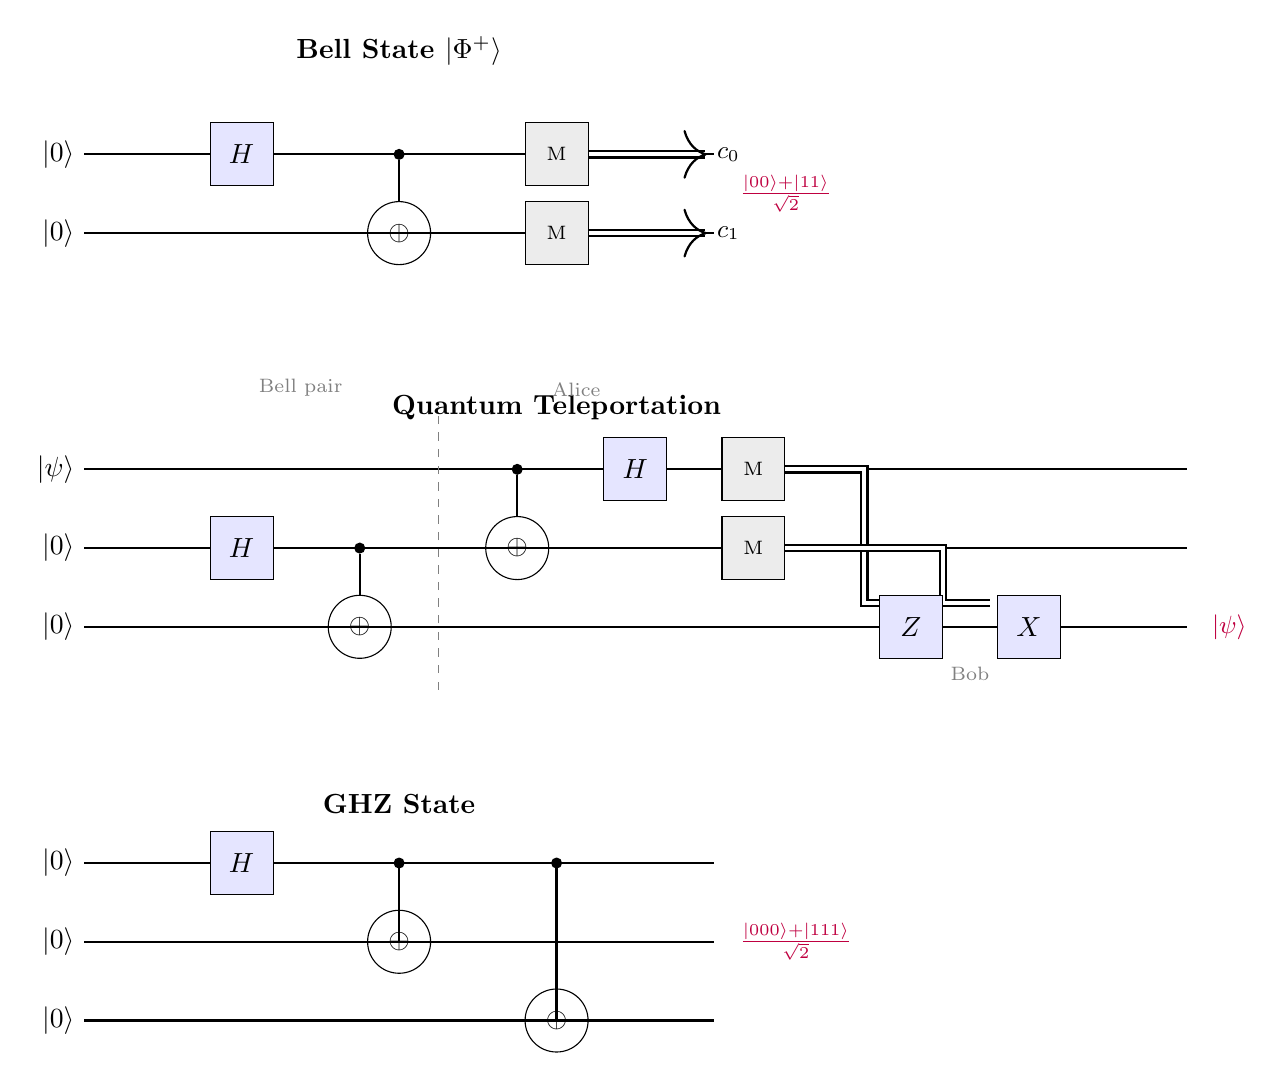
\begin{tikzpicture}[
    gate/.style={draw, fill=blue!10, minimum size=8mm, font=\normalsize},
    meas/.style={draw, fill=gray!15, minimum size=8mm, font=\normalsize},
    ctrl/.style={circle, fill=black, inner sep=0pt, minimum size=4pt},
    targ/.style={circle, draw, inner sep=0pt, minimum size=8mm, font=\normalsize},
    wire/.style={thick},
    cwire/.style={thick, double, double distance=1.5pt},
]

% =============================================================================
% Circuit 1: Bell State (EPR pair)
% =============================================================================
\begin{scope}[shift={(0,0)}]
    \node[font=\bfseries, anchor=south] at (4, 2) {Bell State $|\Phi^+\rangle$};

    % Qubit labels
    \node[left] at (0, 1) {$|0\rangle$};
    \node[left] at (0, 0) {$|0\rangle$};

    % Wires
    \draw[wire] (0, 1) -- (8, 1);
    \draw[wire] (0, 0) -- (8, 0);

    % Hadamard gate on q0
    \node[gate] (H) at (2, 1) {$H$};

    % CNOT: control on q0, target on q1
    \node[ctrl] (c) at (4, 1) {};
    \node[targ] (t) at (4, 0) {$\oplus$};
    \draw[thick] (c) -- (t);

    % Measurement
    \node[meas] (m0) at (6, 1) {\rotatebox{0}{\scriptsize M}};
    \node[meas] (m1) at (6, 0) {\rotatebox{0}{\scriptsize M}};

    % Classical wires
    \draw[cwire, ->] (m0.east) -- ++(1.5, 0) node[right, font=\small] {$c_0$};
    \draw[cwire, ->] (m1.east) -- ++(1.5, 0) node[right, font=\small] {$c_1$};

    % Output annotation
    \node[right, font=\small, text=purple] at (8.2, 0.5) {$\frac{|00\rangle + |11\rangle}{\sqrt{2}}$};
\end{scope}

% =============================================================================
% Circuit 2: Quantum Teleportation
% =============================================================================
\begin{scope}[shift={(0, -5)}]
    \node[font=\bfseries, anchor=south] at (6, 2.5) {Quantum Teleportation};

    % Qubit labels
    \node[left] at (0, 2) {$|\psi\rangle$};
    \node[left] at (0, 1) {$|0\rangle$};
    \node[left] at (0, 0) {$|0\rangle$};

    % Wires
    \draw[wire] (0, 2) -- (14, 2);
    \draw[wire] (0, 1) -- (14, 1);
    \draw[wire] (0, 0) -- (14, 0);

    % Step 1: Create Bell pair (q1, q2)
    \node[gate] (H1) at (2, 1) {$H$};
    \node[ctrl] (c1) at (3.5, 1) {};
    \node[targ] (t1) at (3.5, 0) {$\oplus$};
    \draw[thick] (c1) -- (t1);

    % Separator
    \draw[dashed, gray] (4.5, -0.8) -- (4.5, 2.8);

    % Step 2: Alice's operations (q0, q1)
    \node[ctrl] (c2) at (5.5, 2) {};
    \node[targ] (t2) at (5.5, 1) {$\oplus$};
    \draw[thick] (c2) -- (t2);

    \node[gate] (H2) at (7, 2) {$H$};

    % Step 3: Measurements
    \node[meas] (ma) at (8.5, 2) {\scriptsize M};
    \node[meas] (mb) at (8.5, 1) {\scriptsize M};

    % Classical wires to corrections
    \draw[cwire] (ma.east) -- ++(1, 0) |- (10.5, 0.3);
    \draw[cwire] (mb.east) -- ++(2, 0) |- (11.5, 0.3);

    % Step 4: Bob's corrections
    \node[gate] (Z) at (10.5, 0) {$Z$};
    \node[gate] (X) at (12, 0) {$X$};

    % Output
    \node[right, font=\small, text=purple] at (14.2, 0) {$|\psi\rangle$};

    % Labels
    \node[font=\scriptsize, gray, above] at (2.75, 2.8) {Bell pair};
    \node[font=\scriptsize, gray, above] at (6.25, 2.8) {Alice};
    \node[font=\scriptsize, gray, above] at (11.25, -0.8) {Bob};
\end{scope}

% =============================================================================
% Circuit 3: GHZ State
% =============================================================================
\begin{scope}[shift={(0, -10)}]
    \node[font=\bfseries, anchor=south] at (4, 2.5) {GHZ State};

    % Labels
    \node[left] at (0, 2) {$|0\rangle$};
    \node[left] at (0, 1) {$|0\rangle$};
    \node[left] at (0, 0) {$|0\rangle$};

    % Wires
    \draw[wire] (0, 2) -- (8, 2);
    \draw[wire] (0, 1) -- (8, 1);
    \draw[wire] (0, 0) -- (8, 0);

    % H on q0
    \node[gate] (H) at (2, 2) {$H$};

    % CNOT q0→q1
    \node[ctrl] at (4, 2) {};
    \node[targ] at (4, 1) {$\oplus$};
    \draw[thick] (4, 2) -- (4, 1);

    % CNOT q0→q2
    \node[ctrl] at (6, 2) {};
    \node[targ] at (6, 0) {$\oplus$};
    \draw[thick] (6, 2) -- (6, 0);

    % Output
    \node[right, font=\small, text=purple] at (8.2, 1) {$\frac{|000\rangle + |111\rangle}{\sqrt{2}}$};
\end{scope}

\end{tikzpicture}
\end{document}
